
\section{VI - Reconnaissance de mot}
\begin{frame}{VI - Reconnaissance de mot}
	\begin{block}{}
		Le site du gouvernement recense ces mots-clés pour les numéro d'appels d'urgences : \\
		\begin{enumerate}
		  \item[n°15] malaise, hémorragie, brûlure, intoxication
		  \item[n°17] violences, agression, vol, cambriolage
		  \item[n°18] incendie, gaz, effondrement, électrocution
		\end{enumerate}
	\end{block}
\begin{figure}
	\begin{subfigure}[]{0.3\textwidth}
		\includegraphics[width=\textwidth]{1-Incendie.jpg}
  		\caption{INCENDIE}
	\end{subfigure}
	\begin{subfigure}[]{0.3\textwidth}
		\includegraphics[width=\textwidth]{1-Intoxication.jpg}
  		\caption{INTOXICATION}
	\end{subfigure}
	\begin{subfigure}[]{0.3\textwidth}
		\includegraphics[width=\textwidth]{1-Cambriolage.jpg}
		\caption{CAMBRIOLAGE}
	\end{subfigure}
\end{figure}
\end{frame}


\begin{frame}{VI - Transfert d'apprentissage}
	\begin{figure}
		\includegraphics[width=\textwidth]{2-transfert.png}
		\caption{Schéma de fonctionnement du transfert d'apprentissage}
	\end{figure}
\end{frame}


\begin{frame}{VI - }

	

\end{frame}